\RequirePackage{setspace}
\documentclass{ejb}
\setcounter{page}{1} % Please input the first page number in place of "1". This will change the starting page number of the paper.

%       -------------------------------------------------------------------

\usepackage{comment}
\usepackage{rotating}
\usepackage{xspace}
\usepackage{tikzscale}
\usepackage{filecontents}
\usepackage{tikz}
\usepackage{fancyvrb}
%\usepackage{subcaption}
\usepackage{pgfplotstable}
\usepackage{longtable}
\usepackage{pgfplots}
\usepackage{hyperref}
\usepackage{helvet}
\usepackage[eulergreek]{sansmath}
\usepackage{graphicx}
\usepackage{subfig}
\usepackage{pdflscape}
\usepackage{multirow}
\usepackage{fancyhdr}
\usepackage{pdflscape}
\usepackage{amsmath}
\usepackage{amssymb}
\usepackage{relsize}
\pagestyle{fancy}
\chead{\textit{April 2024\\Draft: Do not cite or quote without permission.}}
%\cfoot{\textit{Draft: Do not cite or quote without permission.}}
\renewcommand{\headrulewidth}{0.4pt}

\pgfplotsset{compat=1.3}

\fvset{formatcom=\color{black},fontsize=\scriptsize,frame=single,rulecolor=\color{black},baselinestretch=1,framesep=5mm}
\renewcommand{\FancyVerbFormatLine}[1]{\textcolor{blue}{#1}}
\DefineVerbatimEnvironment {GAMSCode*}{Verbatim}
{framesep=5mm,frame=none,fontsize=\scriptsize, baselinestretch=1}

\newcommand{\cv}{\mbox{\boldmath$c$}}
\newcommand{\pv}{\mbox{\boldmath$p$}}
\newcommand{\GAMS}{\textsc{gams}\xspace}
%       -------------------------------------------------------------------

\graphicspath{{.}}

\begin{document}
\title{International trade in agricultural products at the
{U.S.} state level\footnote{
		The findings and conclusions in this paper are
	those of the authors and should not be construed to represent any
	official USDA or U.S. Government determination or policy. This
	research was supported in part by a cooperative agreement
	(58-3000-0-0035) between the U.S. Department of Agriculture,
	Economic Research Service, and the University of Nebraska at
	Lincoln.}
	}            
\author{\small
Edward J. Balistreri\footnote{
University of Nebraska-Lincoln. (email:
{\texttt edward.balistreri@unl.edu}).}
Thomas F. Rutherford\footnote{
University of Wisconsin.  (email:
rutherford@aae.wisc.edu).} and
Steven S. Zahniser\footnote{
Economic Research Service, USDA.  (email:
steven.zahniser@usda.gov).}
}


%
\maketitle

\begin{abstract}
Abstract:  We develop a structural model that leverages both
input-output accounts and economic-geography to estimate
state-level imports and exports of agricultural products.  We develop
a method that allocates farm revenue across observed exports and
allocates imports across state-level absorption. The model accounts
for economic geography under a gravity theory.  The more proximate
farm output is to observed export nodes, for example, the greater is
the export share.  Our method generates more realistic estimates of
the link between farms, agricultural products, domestic absorption of
these goods, and international trade.  This exercise is a key
component in assessing a given state's exposure to trade shocks.  To
illustrate this we provide descriptive reports that indicate
differences in our estimates relative to other methods.
\end{abstract}

\begin{jelcodes}
F10, C81
\end{jelcodes}

\begin{keywords}
State Trade; Agriculture Exports; Agriculture Imports; State-level
Supply Chains
\end{keywords}

\section{Introduction}

An individual U.S. state's exposure to international markets is often
a topic of social commentary and economic analysis.  Informed
analysis seems to require an estimate of a state's exports and
imports.  Unfortunately, published measures of state-level trade often
fall short of accurately reflecting trade exposure.  U.S. Customs
tracks international trade at specific ports of entry (exit) rather
than the ultimate destination of imports or source of export
shipments. In the official state-trade statistics from the U.S. Census
Bureau too much trade exposure is reported for states with major sea
ports or border crossings, and nearly zero exposure for interior
states producing major export commodities like wheat and soybeans.  An
alternative is to simply share total U.S. exports to states based on
production shares.  While transparent, this method fails to account
for trade costs over economic geography and the co-location embeded in
input-output relationships. 

In this paper we develop and apply a new method for estimating
state-level international trade in agricultural products that
incorporates geographic trade frictions.  The method
is based on a fundamental proposition from trade theory, which posits
equal absorption shares of regionally differentiated goods in the
absence of trade frictions.  Adopting this as an assumption allows us
to calibrate a commodity-specific Armington demand system to
input-output accounts that establish supply and demand vectors for
each state and each port. We then utilize the structure with trade
frictions included to establish the benchmark flows of goods from the
point of production to domestic uses and port-level exports.
Similarly, we distribute port-level imports to their use in specific
states.  While our primary focus is on international trade the method
yields a bilateral interstate trade matrix for each commodity.

Our work complements recent advances in open-source calculations
of state input-output accounts by the Wisconsin National Data
Consortium (WiNDC).\footnote{See \url{https://windc.wisc.edu/}.}
The WiNDC project focuses on publicly available data sources and a
series of routines that generate micro-consistent subnational
accounts.  Previously available subnational accounts where both
expensive and proprietary, which made them less ideal for
research.\footnote{The IMPLAN (\url{https://implan.com/}) state
	accounts are an example of a closed-source commercial
	alternative.}
The academic based WiNDC project has many advantages including its
accessibility, transparency, and extensibility to particular research
questions.  

Representing bilateral interstate and state-level international trade
in the WiNDC accounts remains as a challenge. A lack of reliable data 
on interstate trade favors a \emph{pooled} national market
formulation, which ultimately limits the structural options for
researchers.  At first the U.S. Department of Commerce's Bureau of
Census (Census) reports in the Commodity Flow Survey (CFS) might be
considered the best source for bilateral state trade, but these data
suffer from a fundamental problem.  The CFS tracks shipments of goods not
the goods themselves.  For example, a rail shipment of a bushel of
corn from Eastern Nebraska to Kansas City plus the barge shipment of the
same bushel from Kansas City to New Orleans escalates the quantity
(and value) of the actual corn shipped.  This problem, of double
counting in the CFS data, is noted by \citet{AvW} who
correct the CFS interstate trade flows assuming they are exaggerated
by a factor of 2.08.  Our proposed method for generating bilateral
interstate trade imposes consistency between state-level production
and aggregate absorption and export demand. 

The state-level \emph{international} trade in the core WiNDC accounts is also
a known weakness.  The WiNDC trade data is from Census
reports of imports and exports by state, but these are actually
measured by Port of Entry.\footnote{The Census Bureau 
	disseminates export and import statistics by Port of Entry at
	the HS-6 level \citep{Census}.}  
The port from which agricultural exports exit the United States,
however, are not necessarily or even likely located in the States where
those products are produced.  For instance, corn exports departing the
ports located in the New Orleans Port District were not necessarily
grown in the State of Louisiana.  In fact, the large volume of
Louisiana exports of grains (as reported by Census and thus inferred
in the WiNDC accounts) is only explained by Louisiana's purchase of
grains through the pooled national market.  On the supply side, the
excess supply of corn in a state like Nebraska does not leave its Port
of Entry in Omaha, but rather is absorbed by the pooled national
market.  Looking at the Census data Louisiana exports a significant
quantity of corn but Nebraska, a key corn producer, does not.  A
better representation would attribute international exports (and
imports) of agricultural products to the state of production (and
absorption).  
 
Faced with the problematic Census state-trade data, the U.S.
Department of Agriculture's Economic Research Service (ERS) generates
an alternative measure of state agricultural exports based on cash
receipts.  For these estimates, the products that make up U.S.
agricultural exports are grouped to match the 24 product groups in
U.S. farm sales estimates. For each of these 24 
product groups, U.S. agricultural exports are allocated by State in
approximate proportion to the State's share of national cash receipts
for that product group. Thus, Nebraska, with 12.4 percent (\$8.9
billion) of U.S. cash receipts for corn in 2021, is estimated to have
accounted for 12.6 percent (\$2.3 billion) of U.S. corn exports that
year \citep{USDA_a, USDA_b}. In contrast, the Census Bureau's State Trade Data
indicate Nebraska's corn exports (HS-6 100590) totaled about \$609
million in 2021 \citep{Census}.

Neither of these two estimates are based on a comprehensive
assessment of the use of Nebraska's corn production, along the lines
of USDA's PSD (Production, Supply, and Distribution) Online Database
(U.S. Department of Agriculture, Foreign Agricultural Service, 2023).
Some rough estimates are commonly circulated in the industry,
however. For instance, \citet{Groskopf_Silva} estimate that about
40 percent of Nebraska's 2018 corn crop was used as feedstock for
ethanol production within the State. The \citet{NCBa}
indicates that ``about 16 percent of Nebraska's corn crop is fed to
livestock within Nebraska'' and that ``about 40 percent of the corn
grown in Nebraska is fed to livestock somewhere in the United States
or around the world.'' With respect to exports, the \citet{NCBb}
estimates that international exports account for about 
6 percent of the use of Nebraska's corn production.
          
Our purpose is to inform the key question of how much of a states
production of specific agricultural goods are exported and how much is
disbursed to each of the fifty states (plus D.C.).  We use a
structural gravity model following the theory of \citet{AvW}.  A
presentation of the full theory and its development is given by
\citet{Yotov_etal}.  There are two specific features of this theory
that we leverage in developing our estimates of interstate
agricultural trade and the flows of agricultural products between
ports and states. First is the assumption of identical and homothetic
preferences.  This provides an anchor point for calibration, where in
the absence of trade frictions expenditure shares on regionally
differentiated goods are the same across regions. The second
assumption is that trade cost are of the iceberg type.  That is, they
are paid in units of the good being shipped.  This allows us to
establish trade at normalized prices at both the frictionless anchor
and the benchmark equilibrium. 

The remainder of the paper is organized as follows:  In the next
section we consider the frictionless anchor point suggested in the
gravity theory.  In Section \ref{model} we present our model and
method in the context of the 
structural model.  In Section \ref{data} we itemize the data sources.
Results are presented in Section \ref{results} with a comparison to
other methods and including sensitivity analysis.  Concluding remarks
are offered in section \ref{conclusion}.\\

\section{Gravity Theory and the Frictionless Anchor}
\label{gvtyanchor}

We start by considering a structural gravity model under regionally 
differentiated goods as presented by \citet{AvW} and
\citet{Yotov_etal}.  We generally adopt the notation of
\citet{Yotov_etal} with the exception that we index goods using
$i \in I$ and regions (states) using $s \in S$ or $r \in S$. We
proceed in this section by suppressing the index on the good, which is
consistent with the one-sector general-equilibrium treatment of
\citet{AvW}.  The structure remains intact for each individual
good under \emph{separability} as demonstrated by \citet[Appendix
B]{Larch_Yotov_2016}.\footnote{
	Separability such that each good abides by the fundamental
	one-sector \citet{AvW} gravity system requires additional
	assumptions.  The assumptions made by \citet[Appendix
	B]{Larch_Yotov_2016} are shown to be sufficient.}
Another simplification in the \citet{AvW} theory as presented is the
suppression of intermediate inputs to production.  The extension to
accommodate measured intermediates requires us to consider regional
supply of a good to be measured as gross output (not value added) and
expenditures on the good to include intermediates as
well as final demand---absorption.

A fundamental assumption of the \citet{AvW} structure is an identical
and linearly homogeneous \emph{Armington} aggregation of the regionally
differentiated goods.\footnote{The seminal analysis that viewed
	international trade data as being comprised of regionally
	differentiated goods comes from \citet{Armington_1969}.}
This aggregate is then available for absorption in terms of
intermediate inputs in production and final demand.  Let us denote
supply of this \emph{Armington} aggregate (or composite) in region
$s$ as $A_s$.  Assuming a Constant Elasticity of
Substitution (CES) aggregator we have an analog to equation
(1-1) of \citet[p13]{Yotov_etal}:
\begin{equation}
\label{E:primal}
A_s = \left[\sum_r \alpha_r^{\frac{1-\sigma}{\sigma}}
c_{rs}^{\frac{\sigma-1}{\sigma}}\right]^{\frac{\sigma}{\sigma-1}}.
\end{equation}
This technology is better represented in its dual form as the
\emph{minimized} unit-cost function, which embeds optimal sourcing of
each regional variety. Let $p_r$ indicate the factory-gate price, and
let $t_{rs}$ be the trade cost index associated with shipping from $r$
to $s$.  With no trade costs the $t_{rs}$ would be one.  We also
assume symmetry in trade costs, $t_{rs}=t_{sr}$.  An agent in
region $s$ will minimize expenditures ($\sum_r p_r t_{rs} c_{rs}$)
conditional on $A_s$.  Under linear homogeneity, expenditures (cost) is
linear in $A_s$, so we can choose any scale of $A_s$ to represent the
technology.  Conditional on a scale of one unit ($A_s=1$), the unit-cost 
or, equivalently, the unit-expenditure function is  
\begin{equation}
\label{E:P}
P_s = \left[\sum_r \left(\alpha_r p_r
t_{rs}\right)^{1-\sigma}\right]^{\frac{1}{1-\sigma}}.
\end{equation}
$P_s$ can be interpreted as an ideal price index or equivalently the 
marginal cost of a unit of the composite $A_s$.  The corresponding 
level of expenditures is 
\begin{equation}
\label{E:Exp}
E_s = P_s A_s.
\end{equation}

The remainder of the equilibrium is somewhat mechanical.  
The nominal value of supply, denoted $Y_r$, is given by the product
price and the fixed supply quantity 
\begin{equation}
\label{E:Inc}
Y_r = p_r q_r.
\end{equation}
Demand is derived by applying the envelope
theorem to minimized expenditures and then summing across the
potential destinations.  Market clearance is thus given by 
\begin{equation}
\label{E:mkt}
 q_r = \sum_s A_s \frac{\partial P_s(\pv)}{\partial p_r}.
\end{equation}
It is important to note the operation of so called \emph{iceberg}
transport costs in terms of the market clearance condition.  From the
perspective of the exporter in $r$ the quantity shipped equals
$t_{rs} c_{rs}$ at a price of $p_r$.  From the perspective of the
importer in region $s$ the quantity that arrives for consumption is
$c_{rs}$ at a price of $t_{rs} p_{r}$.\footnote{Conditional demand at
the destination is  
\[c_{rs} = A_s \frac{\partial 
P_s(\pv)}{\partial(p_r t_{rs})},\] 
but at the source it is 
\[t_{rs} c_{rs}=t_{rs} A_s \frac{\partial
P_s(\pv)}{\partial(p_r t_{rs})} = A_s \frac{\partial
P_s(\pv)}{\partial p_r}.\] }

In the context of the one sector \citet{AvW} environment equations
(\ref{E:P})--(\ref{E:mkt}) represent a Walrasian general equilibrium
\citep[see][]{estib}.  In the general equilibrium the quantity
supplied $q_r$ is a fixed endowment quantity, and expenditures are
income ($E_r \equiv Y_r$).  With $n$ regions there are $4n$
equilibrium conditions and $4n$ variables interpreted as follows:
$Y_r$ is nominal income; $A_r$ is an index on welfare; $P_r$ the
true-cost-of-living index, and $p_r$ is the endowment price at its
origin.  We have a Walrasian equilibrium so a unique solution
requires a price normalization.

The focus in the structural gravity literature is on nominal
bilateral trade. To be concrete, under our CES assumption, we can pull
out a bilateral trade term from the right-hand side of the market
clearance condition (\ref{E:mkt}).  In nominal terms this is
\begin{equation}
\label{E:bilat1}
x_{rs} = p_r A_s \frac{\partial P_s(\pv)}{\partial p_r}.
\end{equation}
Taking the derivative and converting this to uncompensated demand
(using $Y_s = E_s = P_s A_s$ from equation \ref{E:Exp}) we have 
\begin{equation}
\label{E:bilat2}
x_{rs} = Y_s \left(\frac{\alpha_r p_r t_{rs}}{P_s}\right)^{1-\sigma}.
\end{equation}
Using equations (\ref{E:Inc}) and (\ref{E:mkt}) nominal market
clearance can be represented as 
\begin{equation}
\label{E:nommkt}
Y_r = \sum_s Y_s \left(\frac{\alpha_r p_r t_{rs}}{P_s}\right)^{1-\sigma}.
\end{equation}
Dividing through by total nominal supply $Y^w \equiv \sum_r Y_r$ and
factoring out the price-weighted source region preference we have
\begin{equation}
\label{E:factor}
\frac{Y_r}{Y^w} = (\alpha_r p_r)^{1-\sigma} \sum_s \frac{Y_s}{Y^w} \left(\frac{
t_{rs}}{P_s}\right)^{1-\sigma},
\end{equation}
To simplify the exposition define the following source-region index as in
\citet{AvW}:  
\begin{equation}
\label{E:Pi}
\Pi_r \equiv \left[\sum_s \frac{Y_s}{Y^w}
\left(\frac{t_{rs}}{P_s}\right)^{1-\sigma}\right]^{\frac{1}{1-\sigma}},
\end{equation}
so equation (\ref{E:factor}) is given as 
\begin{equation}
\label{E:factor2}
\frac{Y_r}{Y^w} = (\alpha_r p_r)^{1-\sigma} \Pi^{1-\sigma}.
\end{equation}
Using this equation to substitute the price-weighted preference
parameters out of equation (\ref{E:bilat2}) give us the fundamental
structural gravity equation \citep{AvW}:
\begin{equation}
\label{E:bilat3}
x_{rs} = \frac{Y_r Y_s}{Y^w} \left(\frac{t_{rs}}{\Pi_r P_s}\right)^{1-\sigma}.
\end{equation}
The structural gravity system used to analyze bilateral trade would
include the gravity equation (\ref{E:bilat2}), as well as the indexes
specified in equations (\ref{E:P}) and (\ref{E:Pi}).  \citet{AvW}
discuss these indexes in terms of inward multilateral resistance
($P_r$) and outward multilateral resistance ($\Pi_r$).  The product of
the inward and outward indexes reflect the fact that, in addition to
the specific bilateral trade cost on the link in question, the trade
flow on that link is impacted by the exporter's relative access to
all markets and the importer's relative access to all markets. 

For our purpose in this paper a key lesson from the structural gravity
system is the fact that in the absence of trade frictions each region
will consume its global expenditure share of goods from any source
region. If we impose $t_{rs}=1 \;\; \forall rs$ so all regions face
the same price vector and therefore the same price index $P_s = P^w
\;\; \forall s$.  Furthermore, with no trade frictions, equation
(\ref{E:Pi}) indicates that the $\Pi_r$ are also invarient across
regions ($\Pi_r = \Pi^w \;\; \forall r$). Nominal trade in the 
absence of frictions is thus 
\begin{equation}
\label{E:xnot}
x_{rs} = \frac{Y_r Y_s}{Y^w} \Gamma,
\end{equation}
where $\Gamma \equiv (\Pi^w P^w)^{\sigma-1}$.  The only way that
equation (\ref{E:xnot}) satisfies market clearance is if $\Gamma = 1$
when there are no trade frictions:
\[\sum_s x_{rs} = Y_r \frac{\sum_s Y_s}{Y^w} = Y_r.\]

To conclude our discussion of the frictionless anchor for calibration
define $\theta_s = Y_s/Y^w$ such that nominal trade flows under no
trade frictions equals the nominal supply weighted by the expenditure
share
\begin{equation}
x_{rs} = \theta_s Y_r;
\end{equation}
or equivalently expenditures at the destination weighted by the supply
share
\begin{equation}
x_{rs} = \theta_r Y_s.
\end{equation}
Calibration of a model consistent with the theory to the frictionless
equilibrium only requires measures of nominal supply in $r$ and
nominal absorption in $r$.  With the model calibrated to the implied
bilateral trade at the frictionless anchor we can use a well
specified gravity system, 
like equations (\ref{E:P})--(\ref{E:mkt}), to estimated bilateral 
trade flows conditional on any set of bilateral trade costs.  Of
course, in a model with states trading with other states and ports
(which facilitate trade with the rest of the world) the structure
must be extended beyond the simple \citet{AvW} model.   

\section{Structural Model}
\label{model}
In this section we develop a structural gravity model in the spirit of
the canonical theory presented above.  We use this structure to 
attributes a state's measured production of an agricultural product,
like wheat (\textsc{wht}), to port-level exports or absorption by one
of the 51 US regions (50 states plus DC).  Similarly, the model
simultaneously allocates port-level imports to each of the 51 US
regions.  To set up the model let us index commodities by $i \in I$.
As a first pass we focus on the 11 aggregate agricultural goods in
the 43 sector GTAP-WiNDC accounts:

\vspace{5pt}
\begin{tabular}{ll}
\textsc{c\_b}&Sugar cane, sugar beet\\
\textsc{ctl}&Bovine cattle, sheep, goats and horses\\
\textsc{gro}&Cereal grains nec\\
\textsc{oap}&Animal products nec\\
\textsc{ocr}&Crops nec\\
\textsc{osd}&Oil seeds\\
\textsc{pdr}&Paddy rice\\
\textsc{pfb}&Plant-based fibers\\
\textsc{v\_f}&Vegetables, fruit, nuts\\
\textsc{wht}&Wheat, and\\
\textsc{wol}&Wool, silk-worm cocoons.\\
\end{tabular}
\vspace{5pt}

\noindent US states are indexed by $s
\in S$ or $r \in S = \{\mbox{AL, AK, AZ,} \ldots\mbox{, WY}\}$.  In
addition, we observe imports and exports at a Port of Entry.  We index
the 40 ports by $k \in K$ as listed:

\vspace{5pt}
\begin{tabular}{lllll}
\textsc{ak\_anch}&Anchorage&&		\textsc{al\_mobi}&Mobile	     \\
\textsc{md\_balt}&Baltimore&&		\textsc{la\_newo}&New Orleans	     \\
\textsc{ma\_bost}&Boston&&		\textsc{ny\_newy}&New York City	     \\
\textsc{ny\_buff}&Buffalo&&		\textsc{az\_noga}&Nogales	     \\
\textsc{sc\_char}&Charleston&&		\textsc{va\_norf}&Norfolk	     \\
\textsc{il\_chic}&Chicago&&		\textsc{ny\_ogde}&Ogdensburg	     \\
\textsc{oh\_clev}&Cleveland&&		\textsc{nd\_pemb}&Pembina	     \\
\textsc{or\_colu}&Columbia-Snake&&	\textsc{pa\_phil}&Philadelphia	     \\
\textsc{tx\_dall}&Dallas-Fort Worth&&	\textsc{tx\_prta}&Port Arthur	     \\
\textsc{mi\_detr}&Detroit&&		\textsc{me\_port}&Portland	     \\
\textsc{mn\_dulu}&Duluth&&		\textsc{ri\_prov}&Providence	     \\
\textsc{tx\_elpa}&El Paso&&		\textsc{ca\_sand}&San Diego	     \\
\textsc{mt\_grea}&Great Falls&&		\textsc{ca\_sanf}&San Francisco	     \\
\textsc{hi\_hono}&Honolulu&&		\textsc{ga\_sava}&Savannah	     \\
\textsc{tx\_hous}&Houston-Galveston&&	\textsc{wa\_seat}&Seattle	     \\
\textsc{tx\_lare}&Laredo&&		\textsc{vt\_stal}&St. Albans	     \\
\textsc{ca\_losa}&Los Angeles&&		\textsc{mo\_stlo}&St. Louis	     \\
\textsc{fl\_miam}&Miami&&		\textsc{fl\_tamp}&Tampa		     \\
\textsc{wi\_milw}&Milwaukee&&		\textsc{dc\_wash}&Washington		\\
\textsc{mn\_minn}&Minneapolis&&		\textsc{nc\_wilm}&Wilmington.        
\end{tabular}
\vspace{5pt}

\noindent As a rule we will assume that there is a well defined
mapping from the farm cash-receipts commodity $i$ and an aggregation
of the (six-digit) trade and demand data in the GTAP classification,
so that $i$ refers to both.  

The goal of our exercise is to estimate the following flows of goods between states
and ports:\\
\vspace{5pt}
\begin{tabular}{ll}
$\hat{X}_{irs}$& The bilateral flow of commodity $i$
from state $r$ absorbed in state $s$,\\
$\hat{E}_{irk}$& Exports of commodity $i$ from state
$r$ through port $k$; and\\
$\hat{M}_{ikr}$& Imports of commodity $i$ at port $k$ absorbed in state $r$.
\end{tabular}\\
The challenge is that we have limited data. In the GTAP-WiNDC
state-level input-output accounts we observe the value of absorption
of good $i$ in each state, denoted here as the product of the price
index and composite good: $P_{is} A_{is}$.  Total absorption is
consistent with the state-level use of good $i$ in intermediates and
final demand.  We also observe cash receipts from supply in state 
$r$ as $p^y_{ir} Y_{ir}$, where $Y_{ir}$ is the output quantity and
$p^y_{ir}$ is the factory gate price.  We also observe the value of
imports and exports of good $i$ at port $k$ as $M_{ik}$ and $E_{ik}$.
These observations of the totals discipline the estimated flows
through the following accounting identities:   
\begin{equation}
	P_{is} A_{is} \equiv \sum_r \hat{X}_{irs}  + \sum_k
	\hat{M}_{iks}.
\label{E:absorp}
\end{equation}
In words, the value of observed absorption of good $i$
for intermediate use or final demand in region $s$ ($P_{is} A_{is}$)
is the same as the value of demand of $i$ from all states $r$
(including $r=s$) and all imports allocated to $s$ from ports $k$.
Next we have an identity that indicates market clearance for output
from region $r$.  The value of output of $i$ from $r$ ($p^w_{ir}
Y_{ir}$) is exhausted on shipments to other states and ports of
export. 
\begin{equation}
	p^w_{ir} Y_{ir} \equiv \sum_s \hat{X}_{irs}  + \sum_k \hat{E}_{irk}.
\end{equation}
For international trade we equates the value of total imports of good
$i$ at port $k$ with its estimated disbursement to states $r$
\begin{equation}
	M_{ik} \equiv \sum_r \hat{M}_{ikr};
\end{equation}
and the total value of exports at port $k$ must equal the value of
shipments to that port from across the states $r$
\begin{equation}
	E_{ik} \equiv \sum_r \hat{E}_{irk}.
\label{E:export}
\end{equation}
These linear relationship establish consistency of the solution
estimates, but we need a structural model to translate the observed
data, on the right-hand side of (\ref{E:absorp})--(\ref{E:export}),
into the estimated component flows.

Like the relatively simple model in Section \ref{gvtyanchor}, we build
the structural model around the unit-cost function for
\emph{Armington} aggregation.  As an empirical tool, however, we
specify a more complex nested CES structure.  For a state $s$ absorbing
Armington good $A_{is}$ the relevant components include goods $i$
produced in that state, goods $i$ produced in other states $r \neq s
\in S$, and goods $i$ imported from ports $k \in K$.  Let us denote
the relevant prices $p^y_{ir}$ as the factory-gate price of good $i$
in any state $r$, and $p^m_{ik}$ as the price of import $i$ landed
(import-duty paid) at port $k$.  The unit-cost of $A_{is}$ is given by
\begin{align}
\begin{split}
P_{is} =& \left[\left(\theta_{s}
(t_{ss} p^y_{is})^{1-\sigma_{ln}}+ 
                \left[\sum_{r \neq s} 
		\theta_{r} 
		(t_{rs}
		p^y_{ir})^{1-\sigma_{nn}}
		\right]^{\frac{1-\sigma_{ln}}{1-\sigma_{nn}}} 
\right)^{\frac{1-\sigma_{dm}}{1-\sigma_{ln}}} \right.\\
&\left.+ 
\left(\sum_k 
	\theta_{ik} 
		(t_{ks}
		p^m_{ik})^{1-\sigma_{mm}})^{\frac{1-\sigma_{dm}}{1-\sigma_{mm}}}
\right)^{\left(\frac{1-\sigma_{dm}}{1-\sigma_{mm}}\right)}
\right]^{\frac{1}{(1-\sigma_{dm})}}.
\end{split}
\label{E:zprf_AD}
\end{align}
In the first line of (\ref{E:zprf_AD}) we have a CES aggregation of the
local state good with the national aggregate of other U.S. state
goods at an elasticity of substitution $\sigma_{ln}$.  The national
aggregate of other U.S. state goods has a CES across goods of
$\sigma_{nn}$.  In the second line we have the CES aggregation of imports
from different ports, where the elasticity of substitution is
$\sigma_{mm}$.  This nesting structure gives us considerable flexiblity
in terms of different substitution opportunities among the various
components, and facilitates our ability to perform sensitivity
analysis.  Note, however, that if $\sigma =
\sigma_{ln}=\sigma_{nn}=\sigma_{mm}$ the nesting collapses and we
revert to the simple price index suggested in equation (\ref{E:P})
elaborated with ports as additional sources and destinations.

In (\ref{E:zprf_AD}) we replaced the parameters $\alpha_r$ in the
earlier theory with standard good-specific CES weights $\theta_{ir}$
and $\theta_{ik}$.  While there is a simple conversion back to the
implied $\alpha$, the $\theta$ are more convinient in the context of
calibrating to the frictionless flows. To illustrate, let us choose
supply-quantity units at the frictionless equilibrium such that all
source prices are one ($p_{ir} = p_{kr} =  1$).  Then if we normalize
such that $\sum_r \theta_{ir} + \sum_k \theta_{ik} = 1$ we can see that the
value of the price index must also be one without trade friction
($P_s = 1 \;\; \forall s$).  Furthermore it is relatively easy to see
that, dispite our elaborate nesting, bilateral nominal demand is given
by 
\begin{align}
x_{irs} &= \theta_{ir} P_{is}A_{is} \;\; {\mbox{and}} \\
x_{iks} &= \theta_{kr} P_{is}A_{is}; 
\end{align}
where 
\[
\theta_{ir} \equiv \frac{Y_{ir}}{\sum_s Y_{is}}
		\left[\frac{\sum_s Y_{is}-\sum_k,E_{ik}}{
		\sum_s Y_{is} + \sum_k M_{ik}-\sum_k,E_{ik}}\right], \mbox{and}
\]
\[
\theta_{ik} \equiv\frac{M_{ik}}{\sum_k M_{ik}} \left[
	\frac{\sum_k M_{ik}}{\sum_s Y_{is} + \sum_k M_{ik}-\sum_k,E_{ik}}\right].
\]
While the frist term in each of these fractions is simply the share of
production by state and imports by ports they need to be corrected by
the other terms.  The second term in the first definition is the share
of total US non-exported output to total US absorption.  The second term in the
second definition is the share of total imports in US absorption.
With these weights was have as indicated before $\sum_r \theta_{ir} +
\sum_k \theta_{ik} = 1$.  The key is that these are now indicated by
the observable data indicating uniform consumption of the regionally
differentiated goods in the absence of friction.

We still need to develop the state-level export demand system which
ships to ports that portion of output that is not absorbed in the US.
Let us again use the notion of Armington aggregation to specify the
port-specific unit cost, $P^x_{ik}$ of exporting some good $i$ from port
$k$:
\begin{equation}
\label{E:ExpP}
P^x_{ik} = \left(\sum_r
\theta^x_{ir}(t_{rk}p^y_{ir})^{1-\sigma_x}\right)^{\frac{1}{1-\sigma_x}},
\end{equation}   
where the $\theta^x_{ir} = \frac{Y_{ir}}{\sum_s Y_{is}}$ are simply
the production shares.  Again with no frictions and all price at one
the nominal export demand at a port is just the state production share
times the level of port exports:
\begin{equation}
e_{irk} = \theta^x_{ir} E_{ik}
\end{equation}

Away from the frictionless equilibrium we have to hold the $\theta$
parameters fixed and calculate estimated 
bilateral inter-state trade, state imports, and state export.  These
can be calculated at an equilibrium based on the nominal demand
functions implied by the unit expenditure function (\ref{E:zprf_AD}):
\begin{equation}
\hat{X}_{irs} = p^y_{ir} P_{is} A_{is} \frac{\partial P_{is}(\pv)}{p^y_{ir}},
\;\; {\mbox and,}
\label{E:xhat}
\end{equation}
\begin{equation}
\hat{M}_{iks} = p^m_{ik} P_{is} A_{is} \frac{\partial
P_{is}(\pv)}{p^m_{ik}},
\;\; {\mbox and,}
\label{E:mhat}
\end{equation}
Conditional on trade costs these two equations provide the disposition
of imports and bilateral trade.  On the export demand side we make a
similar calculation based on the unit cost of exporting at a given
port.  State level exports using the demand functions derived from
(\ref{E:ExpP}) are
\begin{equation}
\label{E:ExpbySt}
\hat{E}_{isk} = p^y_{is} E_{ik} \frac{\partial P^x_{ik}(\pv)}{\partial p^y_{is}}.
\end{equation} 

We can close the system by using these demand function and the data
identities to specify the market clearance conditions.  We maintain
the observed total values as given by the right-hand sides of
equations (\ref{E:absorp})--(\ref{E:export}) in both the equilibrium
with frictions and in the frictionless anchor. In this regard we are
adopting the \emph{conditional general equilibrium} environment
suggested by \citet[p75]{Yotov_etal}.    

\section{Data}
\label{data}
\begin{enumerate}
	\item USDA Cash receipts.
	\item Census port-level trade.
	\item Physical distance: State to state and state to port.
	\item GTAP-WiNDC Accounts.
	\item Trade costs.
	\item Elasticities.
\end{enumerate}

\section{Results}
\label{results}

\begin{table}
\caption{State exports of Soybeans (OSD)}
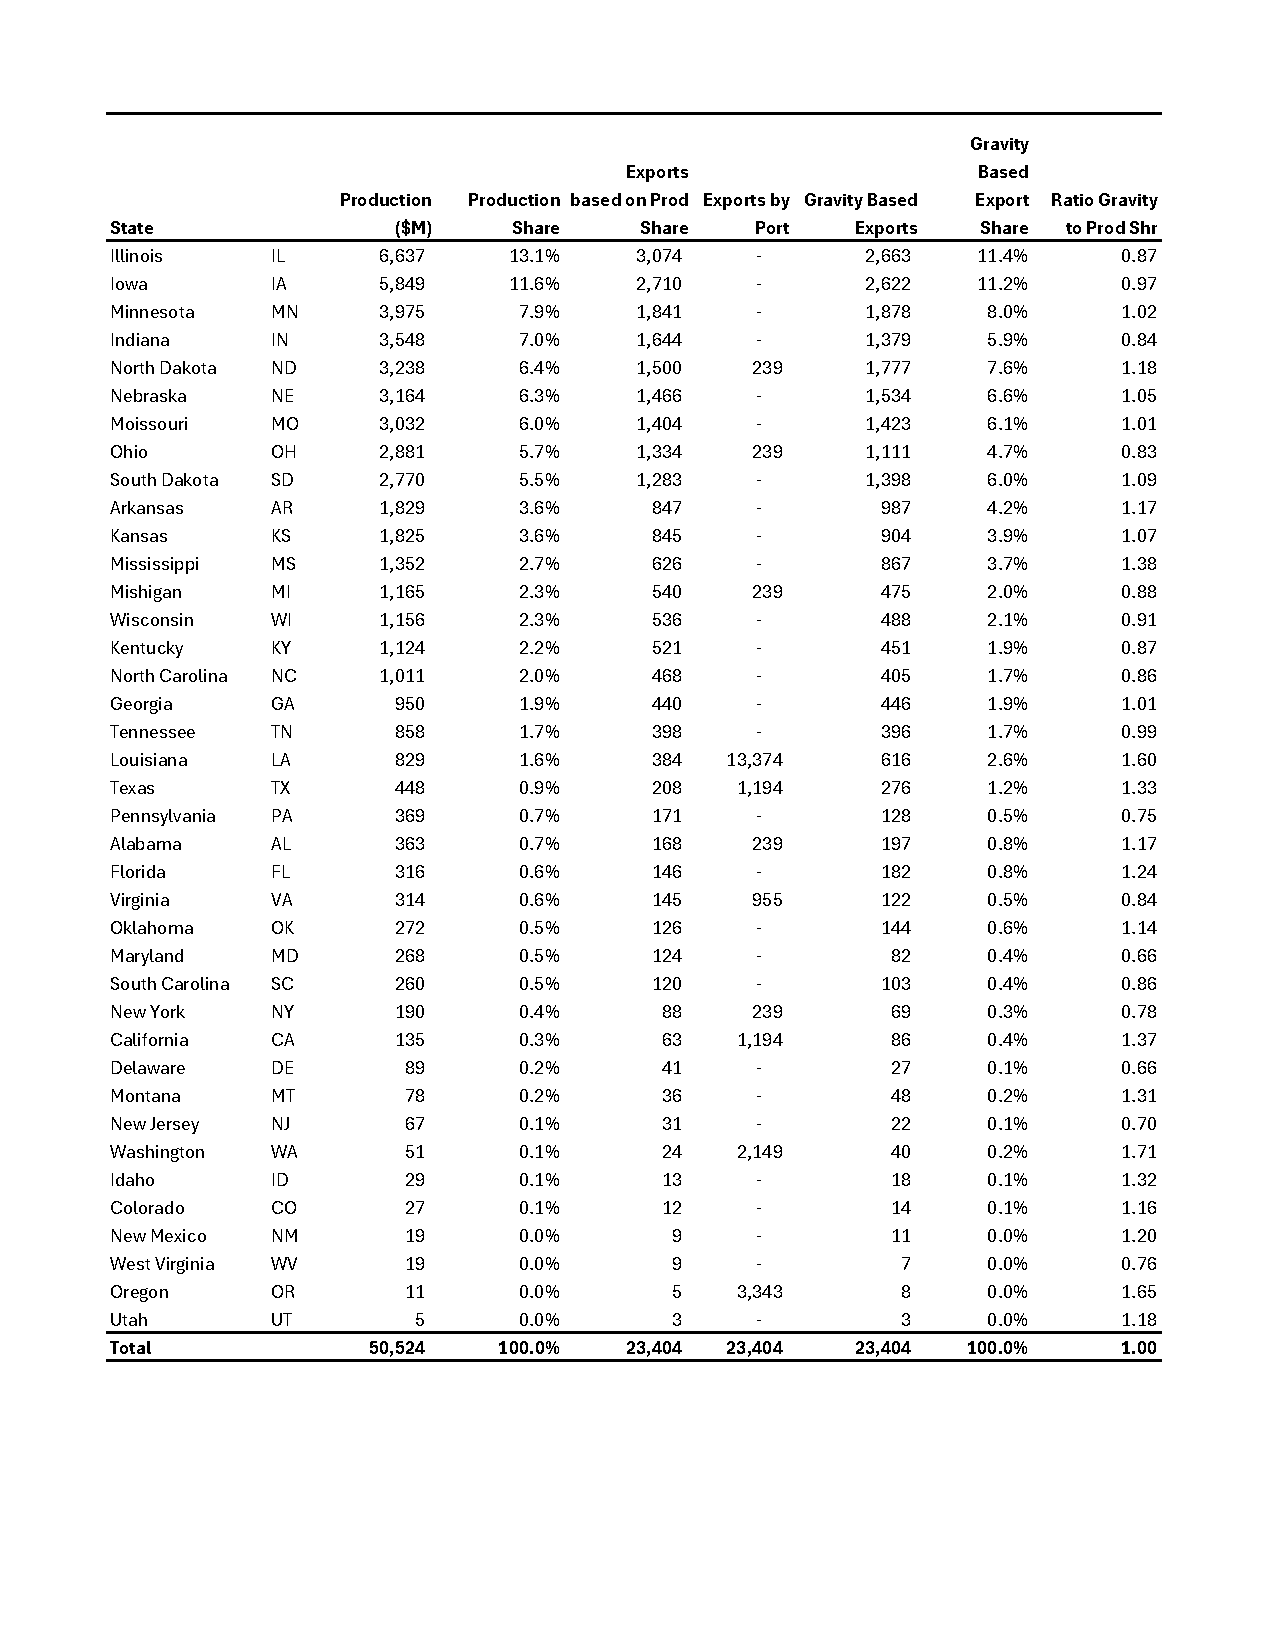
\includegraphics[scale=0.7]{Soybeans.pdf}
\end{table}

\begin{table}
\caption{State exports of Wheat (WHT)}
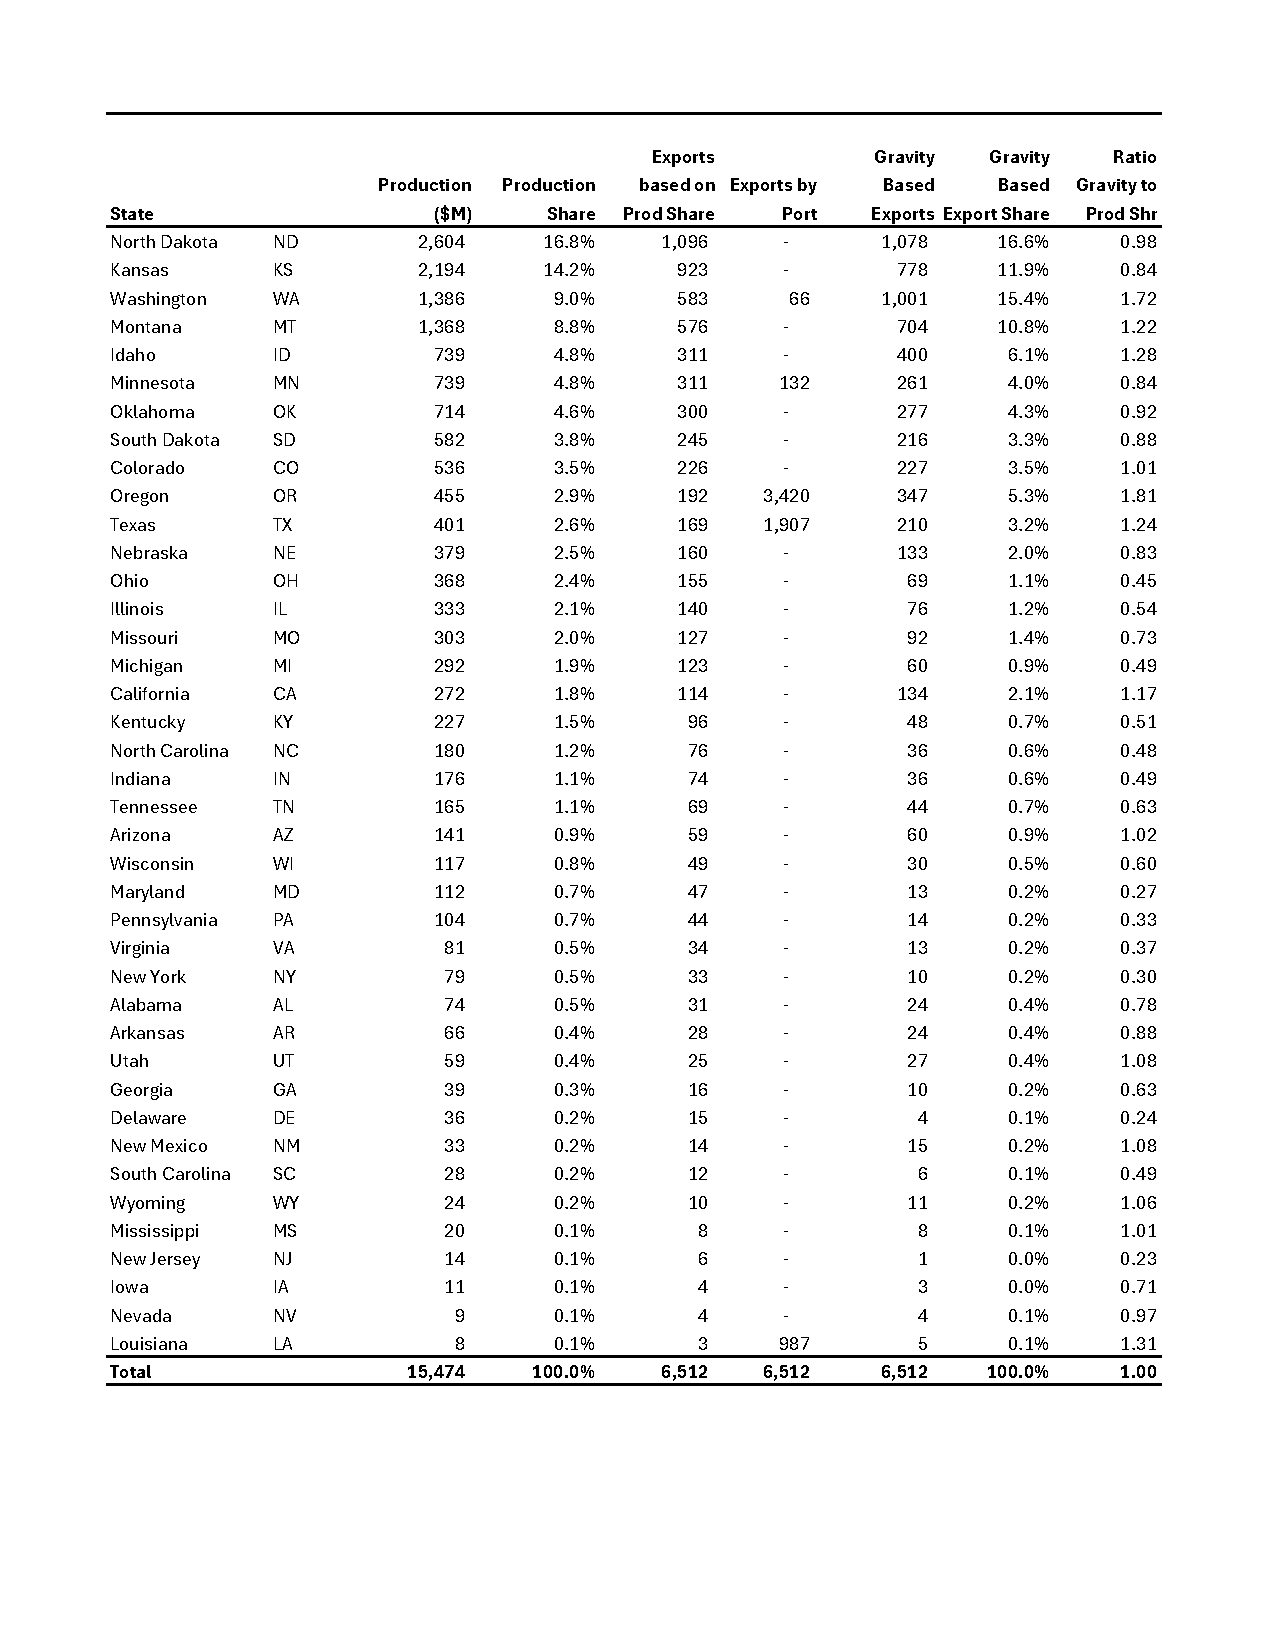
\includegraphics[scale=0.7]{Wheat.pdf}
\end{table}

\newpage
\begin{comment}
Preliminary calculations based on these two models are intriguing,
demonstrating that ATM estimates in the bilateral model are much smaller
than ATM estimates in the corresponding pooled model.  We are looking
forward to finding an intuitive explanation for these results in the
next few months.  \textit{N.B. We cannot rule out the most likely
explanation, i.e. a bug in the calculation!}


\medskip

\textbf{National ATM Estimates: Pooled versus Bilateral Model}
\begin{center}
\includegraphics[width=0.75\textwidth]{Pooled_Bilateral.png}
\end{center}

\newpage

\textbf{ATM Estimates by State: Pooled Model}

\begin{center}
\begin{tabular}{cc}
Pooled Model & Bilateral Model \\
\hline \\
\includegraphics[width=0.45\textwidth]{Pooled.png} &
\includegraphics[width=0.45\textwidth]{bilateral.png}
\end{tabular}
\end{center}
\end{comment}

\section{Conclusion}
\label{conclusion}

This analysis contributes to the...\\

\singlespacing
\begin{acknowledgements}
	The findings and conclusions in this paper are
	those of the authors and should not be construed to represent any
	official USDA or U.S. Government determination or policy. This
	research was supported in part by a cooperative agreement
	(58-3000-0-0035) between the U.S. Department of Agriculture,
	Economic Research Service, and the University of Nebraska at Lincoln.
\end{acknowledgements}

\newpage
\bibliographystyle{jgea}
\bibliography{USDA_bib.bib}
\end{document}
